\documentclass[letterpaper,twocolumn,10pt]{article}
\usepackage{usenix,epsfig,endnotes}
\usepackage{hyperref}
\usepackage{listings}
\usepackage{xcolor}
\usepackage{graphicx}
\usepackage{booktabs}

\begin{document}

\date{}

\title{\Large \bf CS-412 Software Security: Fuzzing libpng}

\author{
  {\rm Louis Gogniat} \and
  {\rm Donia Gasmi} \and
  {\rm Srushti Singh} \and
  {\rm Khaled Kerouch}
}

\maketitle
\thispagestyle{empty}

\subsection*{Abstract}
Image parsing libraries have emerged as compelling targets for fuzzing due to their widespread deployment, continuous exposure to untrusted inputs, and long history of parser-driven memory-safety vulnerabilities. In this work, we present a coverage-guided fuzzing campaign against \texttt{libpng}~1.2.52, the reference C implementation of the PNG image format. Using AFL++ with compile-time instrumentation and AddressSanitizer, we built a harness targeting the full PNG decoding pipeline,
assembled a format-aware seed corpus, and ran both an instrumented and a QEMU-mode (binary-only) campaign for one hour each. Our standard campaign discovered 24 unique crashes, all caused by a
\texttt{stack-use-after-scope} bug in \texttt{png\_inflate()}
(\texttt{pngrutil.c}), reachable via both \texttt{iCCP} and
\texttt{zTXt} chunk handlers. The bug was silently fixed in libpng~1.2.53.

\section{Introduction}

Fuzzing is one of the most effective techniques for finding
memory-safety bugs in C libraries that parse untrusted binary
input. We target libpng library which parses a richly structured
binary format with CRC-protected chunks, zlib-compressed data streams,
and a complex transformation pipeline, all of which constitute deep
attack surface. Several historical CVEs in libpng were originally
found by fuzzing, making it a well-motivated target. We intentionally
chose version~1.2.52 over the latest release to increase the
likelihood of finding real bugs while keeping the methodology sound. Finally, we examine the effect of persistent mode execution on fuzzing performance and discuss how instrumentation depth and sanitizer overhead influence overall campaign efficiency.

\section{Q1 --- Harness Design}
\label{sec:q1}

\subsection{Entry-Point Selection}

We targeted the full PNG \emph{decoding} pipeline via
\texttt{png\_read\_info} followed by \texttt{png\_read\_image}.
This call sequence exercises the complete parser: signature
validation, chunk dispatch, IHDR field parsing, ancillary chunk
handling (iCCP, bKGD, tEXt, tRNS), zlib decompression, and scanline
defiltering. Several notable CVEs including CVE-2015-8126 and
CVE-2016-10087 were triggered through this path, making it the most
security-relevant entry point.


We considered two other alternatives. The \emph{encoder} pipeline (\texttt{png\_write\_image}) would also have been an attractive fuzzing target. The encoder operates on the pixel layout produced by the decoder. This is interesting because encoder routines are generally not designed to defensively handle inconsistent internal state originating from malformed decoder outputs. We ultimately prioritized the decoder because it is more directly exposed to attacker-controlled inputs in real-world deployments. We also considered the simplified high-level API (\texttt{png\_image\_begin\_read\_from\_memory}), which is commonly used in modern applications due to its ease of integration and abstraction over the lower-level decoding pipeline, making bugs here high-impact. However, this API was introduced in libpng~1.6.0 and is therefore unavailable in our target version, libpng~1.2.52.

\subsection{Data Flow and Guards}

The harness accepts input via \texttt{stdin} (instrumented campaign,
no \texttt{@@} in the \texttt{afl-fuzz} invocation) or as a file
path in \texttt{argv[1]} (QEMU campaign, invoked with \texttt{@@}).
Input is read into a heap buffer, and a custom I/O callback
(\texttt{read\_fn}) is registered via \texttt{png\_set\_read\_fn}
so that libpng reads from memory rather than a \texttt{FILE*}.

A key design decision was synthetic signature injection: the callback prepends the valid 8-byte PNG signature before splicing in fuzz data. This prevents AFL++ from wasting mutations on the fixed signature bytes, which libpng validates immediately and which yield no additional coverage when corrupted. An earlier version rejected invalid signatures using \texttt{png\_sig\_cmp}, but this caused rapid coverage stagnation because mutations affecting the signature never reached the parser.

The harness executes both the pull API (\texttt{pngread.c}) and push API (\texttt{pngpread.c}) on every input, as the two parsers share little implementation logic and expose distinct attack surfaces. The pull model targets synchronous file parsing, while the push model exercises incremental streaming logic where chunk boundaries may appear at arbitrary offsets. Restricting fuzzing to a single parser would therefore leave half the attack surface untested. To maximize decoder coverage, five transformation routines are enabled in the pull path, followed by \texttt{png\_read\_update\_info()} to apply the registered transforms to the info struct so that rowbytes reflects the post-transform row size.

A \texttt{setjmp} recovery block surrounds all libpng calls because the library reports errors through \texttt{longjmp}; without a valid jump target, malformed inputs would appear as crashes and flood AFL++ with false positives. Finally, dimension guards (\texttt{height > 5000} or \texttt{rowbytes > 10,000,000}) prevent pathological allocations from mutated headers, while validation of \texttt{fread()} results avoids harness-induced memory errors unrelated to libpng itself.

\section{Q2 --- Instrumentation and Sanitizers}

\label{sec:q2}

libpng was compiled with \texttt{afl-clang-fast},
\texttt{-fsanitize=address -g -O1}, and \texttt{--disable-shared}.
\newline
\\
\texttt{afl-clang-fast} inserts AFL++ edge-coverage callbacks at
compile time. Without it, AFL++ cannot observe which branches a test
case exercises and falls back to blind mutation.

\texttt{-fsanitize=address} is what made crashes visible. The bug in
\texttt{png\_inflate()} is a \texttt{stack-use-after-scope}: without
ASan the invalid stack read produces no signal. This was not
theoretical; our no-sanitizer fork campaign (Q8, 8.83M execs) and QEMU campaign (Q7, 1.78M execs) both found zero crashes.

\texttt{-O1} over \texttt{-O0}: we chose \texttt{-O1} instead of \texttt{-O0} after evaluating their impact through identical 1-hour campaigns using a simplified harness. The \texttt{-O0} configuration achieved an average throughput of approximately 220 exec/sec, decreasing to around 130 exec/sec by the end of the run, whereas \texttt{-O1} maintained 290.2 exec/sec. This corresponds to an approximately 1.3$\times$ slowdown under \texttt{-O0}, without any observable coverage improvement. Additionally, both configurations identified the same root cause across 15 crashes.


\texttt{--disable-shared} statically links libpng into the harness,
ensuring the instrumented library code is what AFL++ actually sees.

\textbf{CRC patch.} We applied
\\
\texttt{utils/libpng\_no\_checksum/libpng-nocrc.patch}, neutralizing
\texttt{png\_crc\_finish()} in \texttt{pngrutil.c}. Every mutated
chunk fails its CRC-32 check: critical chunks abort via
\texttt{png\_error()}; ancillary chunks are silently discarded.
Either way, mutated bytes never reach the parser. Without the patch,
coverage plateaus immediately. We applied it to both builds so the
instrumented/QEMU comparison isolates emulation overhead only.

\section{Q3 --- Seed Corpus and Dictionary}
\label{sec:q3}


\subsection{Seed Corpus}

We assembled a corpus of 32 PNG seeds covering the major axes of
format variation that libpng branches on internally, split into
two groups.
The first 17 files were hand-crafted to target specific code paths:
\texttt{corrupt.png} immediately exercises error-handling paths;
\texttt{minimal.png} (8-byte signature only) hits the earliest
abort paths; and four seeds were programmatically generated to
target auxiliary chunk handlers --- \texttt{seed\_gama.png}
carries a \texttt{gAMA} gamma chunk (triggering the file-gamma
code path instead of the fallback), \texttt{seed\_unknown.png}
embeds a \texttt{fuZz} ancillary chunk (exercising
\texttt{png\_set\_keep\_unknown\_chunks}), \texttt{seed\_ztxt.png}
places a zlib-compressed \texttt{zTXt} chunk after \texttt{IDAT}
(reaching \texttt{png\_read\_end} rather than
\texttt{png\_read\_info}), and \texttt{seed\_itxt.png} carries an
uncompressed UTF-8 \texttt{iTXt} chunk; the remaining 11 cover the
core format variants (grayscale, RGBA, palette, 16-bit depth,
Adam7 interlacing, tRNS, tEXt chunks, and extreme dimensions).
The remaining 15 seeds were drawn from the official libpng test
suite (\texttt{contrib/pngsuite/}), a collection of reference PNG
files used by the libpng project itself for regression testing.
Keeping all seeds under 200~bytes minimises calibration overhead
and maximises executions per second.

\subsection{Dictionary}

We extended the AFL++ PNG dictionary with three token categories.
\emph{Chunk type names} (\texttt{IHDR}, \texttt{IDAT}, \texttt{IEND},
\texttt{PLTE}, \texttt{iCCP}, \texttt{tEXt}, \texttt{tRNS}, etc.)
are the \emph{terminal symbols} of the PNG chunk grammar; the
4-byte sequences on which libpng's dispatcher branches. Without them
the fuzzer must rediscover each token by random mutation with
probability $2^{-32}$ per position. \emph{Boundary length fields}
(big-endian 4-byte values 0, 1, 13, $2^{32}-1$) stress
length-parsing arithmetic. \emph{IHDR sub-field values} (bit depths
1/2/4/8/16, color types 0/2/3/6, interlace flags 0/1) help AFL++
generate structurally valid headers faster, reaching the deeper
pixel-data pipeline.

From the AFL++ status screen after 33 minutes hour and 1.71M executions, the dictionary shows very limited usage (14 active entries out of ~17.4k–17.7k available), indicating that most dictionary tokens did not significantly contribute to execution guidance. In contrast, the majority of new coverage was driven by havoc and splice mutations, which accounted for most of the exploration of new paths. This suggests that the fuzzing campaign was primarily mutation-driven rather than dictionary-guided, likely because the existing corpus already covered most structured input requirements.

\section{Q4 --- Campaign Analysis}
\label{sec:q4}

We ran the instrumented campaign for 1~hour via \texttt{make fuzz}
with \texttt{interesting\_seeds} and the extended dictionary. All
plots and the status screen are in Appendix~A
(Figures~\ref{fig:status-instrumented}--\ref{fig:exec-speed}).

\textbf{Key metrics} after 1.71M executions: stability 100\%,
corpus count 1201, map density 32.85\%, count coverage
3.72~bits/tuple, cycles done 6, exec speed 855~exec/sec, 24
crashes saved. During fuzzing, 314 new edges were discovered, corresponding to previously unseen control-flow transitions that expanded the coverage map over time. Stability at 100\% confirms the harness is fully deterministic.

\textbf{Edges curve} (Figure~\ref{fig:edges}): the campaign started
at $\sim$300 edges and grew to $\sim$1250, showing three distinct phases; rapid discovery in the first 600s, a slower discovery phase with diminishing
returns around 900 edges from $t$=600--1{,}400s, and a final near-plateau
starting around $t$=1{,}400s where edge growth becomes minimal.

With 427 pending items and only 6 cycles completed, the campaign had
not reached full saturation at the 33-minutes mark. The 32.85\% map
density indicates significant unexplored edges.

\section{Q5 --- Crash Triage}
\label{sec:q5}

AFL++ found 24 unique crashes within the first 33 minutes, all
\texttt{sig:06} (SIGABRT). Triaging all 24 confirmed a single root
cause, triggered via two chunk handlers: \texttt{png\_handle\_zTXt} and \texttt{png\_handle\_iCCP}, both reaching the bug through the shared path
\texttt{png\_decompress\_chunk} $\rightarrow$ \texttt{png\_inflate}.
\newline
\\
\textbf{Reproduction.} The crashing input was reproduced directly
from the AFL++ crash corpus.
% \begin{verbatim}
% ASAN_OPTIONS=symbolize=1 ./png_harness \
%   "findings/default/crashes/id:000000,
%    sig:06,src:000068,..."
% \end{verbatim}
\newline
\\
\textbf{Minimization.} We ran \texttt{afl-tmin}, reducing the input
from 104 to 50~bytes (37.5\% reduction, 196 executions), simplifying
root-cause analysis while preserving the crash trigger.
\newline
\\
\textbf{Root cause.} The bug is a \texttt{stack-use-after-scope} in
\texttt{png\_inflate()} (\texttt{pngrutil.c:306}). A local buffer
\texttt{umsg[52]} is declared inside an inner scope block and
\texttt{msg} is pointed at it. When the block closes, ASan poisons
the stack memory; \texttt{png\_warning(png\_ptr,~msg)} then reads the
dead pointer. The full ASan stack trace is in
Figure~\ref{fig:asan-trace}.

{\small
% \begin{verbatim}
% /* 1.2.52 - buggy */
%   msg = umsg;
% }                     /* umsg destroyed */
% png_warning(ptr, msg);/* reads dead stack */

% /* 1.2.53 - fixed */
%   msg = umsg;
%   png_warning(ptr, msg); /* inside scope */
% }
% \end{verbatim}
}
\noindent
\textbf{Fix.} The bug is present in libpng~1.2.52 and absent in 1.2.53. Comparing the two versions, \texttt{png\_inflate()} was restructured so that \texttt{png\_warning} is called inside the scope block where \texttt{umsg} is declared, rather than after it closes. The exact commit is part of the 1.2.53 beta development cycle (February 2015).

In our experiments, the issue produced no observable crash behaviour without ASan instrumentation. Because the invalid access is limited to a short-lived stack read immediately after scope exit, we believe the issue is likely low severity in practical exploitation terms. Nevertheless, it remains real undefined behaviour and may still lead to unstable behaviour or limited information disclosure depending on compiler optimizations and stack layout.


\section{Q6 --- Attack Surface Analysis}
\label{sec:q6}

\textbf{Mozilla Firefox} uses libpng to decode PNG images embedded
in web pages. A remote attacker can serve a crafted PNG from any
origin; the browser fetches and decodes it automatically without user
interaction, making this a zero-click attack surface reachable from
the open web.

\textbf{Android (Skia graphics library)} links libpng to decode PNG
assets in applications and system UI. A malicious image delivered via
MMS, email attachment, or file download could trigger a decoder bug
within the receiving process. If the vulnerable process runs with
elevated permissions (as system UI processes often do), this could
facilitate privilege escalation.

\textbf{Unexercised code paths.} 
Despite the inclusion of the Progressive API and basic transformations, significant gaps remain in the harness's coverage. First, the harness completely ignores the encoding pipeline (pngwrite.c). While the decoder is the primary entry point for external data, many server-side applications ingest user images, modify them, and then re-encode them. Vulnerabilities in the encoder—such as integer overflows during chunk length calculation or CRC generation—could allow an attacker to compromise a server during the output phase of an image processing pipeline.

Furthermore, the harness does not invoke \texttt{png\_set\_interlace\_handling()}, leaving the complex coordinate-mapping and row-buffer reuse logic for Adam7 interlacing in pngrutil.c unexercised. In legacy versions like libpng 1.2.52, these multi-pass calculations lack modern bounds-checking, making "off-by-one" errors a high-risk source of heap corruption.

\section{Q7 --- Binary-Only Fuzzing (QEMU Mode)}
\label{sec:q7}

We compiled the harness with \texttt{gcc} (no AFL++ instrumentation,
no sanitizers) and ran AFL++ with \texttt{-Q}, using the same seed
corpus and dictionary as the instrumented campaign.
 
\textbf{Coverage mechanism.} In compile-time instrumentation mode,
AFL++ inserts inline callbacks at every branch edge via
\texttt{afl-clang-fast}, updating a shared bitmap in $O(1)$ per
edge with near-zero overhead. In QEMU mode, AFL++ runs the binary
under a modified QEMU user-mode emulator that translates each basic
block from x86 machine code into an intermediate representation on
first encounter, injects coverage tracking, and caches the result.
This translation happens at runtime, adding significant per-instruction
overhead compared to compile-time instrumentation.
 
Table~\ref{tab:comparison} compares both campaigns after 33~minutes.
Plots for the QEMU campaign are in
Figures~\ref{fig:status-qemu}--\ref{fig:qemu-exec-speed}.
 
The edges curve (Figure~\ref{fig:qemu-edges}) started at $\sim$800
and grew continuously to $\sim$3{,}200 over the 33 minutes with no
plateau, contrasting sharply with the instrumented campaign's
three-phase curve. This reflects that QEMU completed only 3 cycles
with 61 pending items. The corpus grew steadily to 1047 entries
(Figure~\ref{fig:qemu-high-freq}), and the pending items
curve started declining towards the end meaning the fuzzer had reached the plateau and there was nothing more interesting left to explore. Exec speed (Figure~\ref{fig:qemu-exec-speed}) averaged
$\sim$890~exec/sec early in the run, declining slightly to
$\sim$300~exec/sec near the end as the corpus declined. The crash/levels graph
(Figure~\ref{fig:qemu-low-freq}) shows zero crashes and zero hangs
throughout, with queue depth growing to 20 levels.
 
% \begin{table}[h]
% \small
% \begin{tabular}{lll}
% \toprule
% \textbf{Metric} & \textbf{Instrumented} & \textbf{QEMU} \\
% \midrule
% Exec speed   & 850/sec  & 890/sec \\
% Total execs  & 1.71M      & 1.78M \\
% New edges    & 314        & 281 \\
% Corpus       & 1201        & 1047 \\
% Map density  & 32.85\%    & 4.83\% \\
% Crashes      & 24         & 0 \\
% Cycles done  & 6          & 3 \\
% \bottomrule
% \end{tabular}
% \caption{Instrumented vs.\ QEMU after 0.5~hour.}
% \label{tab:comparison}
% \end{table}
 
\textbf{Exec speed} was surprisingly higher for QEMU than the instrumented campaign. This is unusual but could be explained by the fact that we ran our campaign on a cluster machine which has much higher memory and CPU throughput. In particular, AddressSanitizer introduces significant shadow-memory overhead that is highly memory-bandwidth intensive; on high-performance hardware, this cost becomes comparatively less dominant. In contrast, QEMU mode remains primarily CPU-bound due to dynamic binary translation overhead, which scales less effectively with increased memory bandwidth.


\textbf{Edge counts} were similar in absolute terms (314 vs.\ 281) but map
density differed dramatically (32.85\% vs.\ 4.83\%): compile-time
instrumentation produces a denser, more accurate coverage map, while
QEMU's runtime translation produces a sparser approximation.
 
\textbf{Crashes.} The QEMU campaign found no crashes after 33~minutes.
The bug is \emph{sanitizer-dependent}:
the \texttt{stack-use-after-scope} produces no OS signal without
ASan, and QEMU mode can only detect crashes generating SIGSEGV or
SIGABRT.
















\section{Q8 --- Instrumentation Depth and Performance}
\label{sec:q8}
\subsection{Instrumented Edge Counts}
 
Using \texttt{AFL\_DEBUG=1}, the libpng library shows multiple
instrumentation outputs across its compilation units, with values
ranging from approximately 13 to 1153 instrumented locations per file.
Aggregating across all files, this corresponds to several thousand
instrumented edges in total.

For the final fuzzing binary, the harness instrumentation reports 53 instrumented locations with no collisions. In addition, AFL++ reports approximately 3803 coverage edges in the final linked executable, corresponding to the full merged coverage map of the harness and all linked libpng code.

These numbers differ because libpng is a large image decoding library with many functions, branches, and error-handling paths, resulting in thousands of instrumented edges; the harness is a minimal wrapper that only calls a small subset of libpng APIs, producing only 53 instrumented locations; and the final value of 3803 represents the total AFL++ coverage map size for the fully linked executable, including the harness, libpng, and all linked runtime components.
 
\subsection{Exec Speed Comparison}
 
Table~\ref{tab:perf} compares exec speed across three
configurations, all using the same harness and seed corpus.
Plots for the no-sanitizer and persistent campaigns are in
Figures~\ref{fig:status-no-asan}--\ref{fig:no-asan-exec-speed}
and Figures~\ref{fig:status-persistent}--\ref{fig:persistent-exec-speed}
respectively.
 
\textbf{No sanitizer vs ASan + fork (4415 vs 855 exec/sec):}
% Removing ASan yields a 5.16$\times$ speedup. ASan instruments
% every memory read and write with shadow memory checks, adding
% per-access overhead that accumulates over millions of executions.
% Without it, the binary runs the same code paths with only
% AFL++'s coverage bitmap overhead. The no-sanitizer campaign
% completed 21 cycles with only 1 pending item; more thorough
% queue processing than the ASan run's 6 cycles and 427 pending,
% a direct consequence of higher throughput. However, it found
% \textbf{zero crashes} despite 8.83M executions, confirming the
% bug is invisible without sanitizer instrumentation.

Disabling ASan yielded a 5.16$\times$ speedup by removing shadow-memory checks on every memory access, leaving only AFL++ coverage instrumentation overhead. The no-sanitizer campaign completed 21 cycles with one pending item, compared to six cycles and 427 pending items for ASan + fork mode. However, despite 8.83M executions, it detected no crashes, showing that the bug was only observable with sanitizer instrumentation.
 
\textbf{ASan + persistent mode (5450 exec/sec, 6.37$\times$ speedup):}
% Persistent mode eliminates \texttt{fork()} overhead by looping
% the harness body 10{,}000 times inside the same process via
% \texttt{\_\_AFL\_LOOP(10000)}. This yielded 10.9M total executions; 6.37$\times$ more than ASan + fork mode's 1.71M in the same
% time. The campaign completed 17 cycles with 0 pending items,
% fully exhausting the queue. 
Persistent mode eliminates repeated \texttt{fork()} overhead by executing the harness loop 10,000 times per process via \texttt{\_\_AFL\_LOOP(10000)}. This increased executions from 1.71M to 10.9M over the same runtime. The campaign completed 17 cycles with zero pending items, fully exhausting the queue.
 
The edges curve (Figure~\ref{fig:persistent-edges}) exhibits a rapid increase to approximately $\sim$1200 edges by $t=300\,\mathrm{s}$, followed by a much slower rise to about $\sim$1260 by $t=1200\,\mathrm{s}$. After this point, the curve remains flat, indicating that the campaign reached full saturation in under 20 minutes. In contrast, the ASan + fork campaign had not yet saturated after 30 minutes.
 
The exec speed graph (Figure~\ref{fig:persistent-exec-speed})
shows 5{,}000--8{,}000 raw exec/sec. The corpus/pending graph
(Figure~\ref{fig:persistent-high-freq}) shows pending items
spiking to $\sim$220 then dropping to near zero by $t$=600s;
the queue was exhausted in under 10~minutes. 77 unique crashes
were found (Figure~\ref{fig:persistent-low-freq}), mostly within
the first 1{,}800s, confirming ASan is active. Stability was
99.92\%, a slight drop from fork mode's 100\%, expected in
persistent mode due to minor state accumulation across iterations.
 










% {\footnotesize \bibliographystyle{acm}
% \bibliography{sample}}

% \newpage
% $~~$
\newpage
\appendix



\section{Instrumented Campaign (Main, Q4)}

\begin{figure}[h]
  \centering
  \includegraphics[width=\columnwidth]{Plots/run1_main_campaign/status.jpeg}
  \caption{AFL++ status screen --- instrumented campaign (ASan + fork, 33 minutes). 850 exec/sec, 24 crashes, 6 cycles, queue not exhausted.}
  \label{fig:status-instrumented}
\end{figure}

\begin{figure}[h]
  \centering
  
\includegraphics[width=\columnwidth]{Plots/run1_main_campaign/edges.png}
  \caption{Edges graph --- instrumented campaign. Edge count grows from
  $\sim$300 to $\sim$1250 with distinct growth phases.}
  \label{fig:edges}
\end{figure}

\begin{figure}[h]
  \centering
  
\includegraphics[width=\columnwidth]{Plots/run1_main_campaign/high_freq.png}
  \caption{Corpus and pending items --- instrumented campaign. Corpus
  grows to 1201; pending items decline as the queue is processed.}
  \label{fig:high-freq}
\end{figure}

\begin{figure}[h]
  \centering
  
\includegraphics[width=\columnwidth]{Plots/run1_main_campaign/low_freq.png}
  \caption{Crashes and queue levels --- instrumented campaign. 24
  unique crashes found; queue depth reached 25 levels.}
  \label{fig:low-freq}
\end{figure}

\begin{figure}[h]
  \centering
  
\includegraphics[width=\columnwidth]{Plots/run1_main_campaign/exec_speed.png}
  \caption{Execution speed --- instrumented campaign. Average
  $\sim$855 exec/sec throughout the run.}
  \label{fig:exec-speed}
\end{figure}

\newpage
$~~$
\newpage
\section{ASan Stack Trace (Q5)}

\begin{figure}[h]
\begin{verbatim}
==ERROR: AddressSanitizer: stack-use-after-scope
READ of size 1 at 0x7ffdef56d3a0
  #0 png_default_warning  pngerror.c:318
  #1 png_warning          pngerror.c:132
  #2 png_inflate          pngrutil.c:306
  #3 png_decompress_chunk pngrutil.c:338
  #4 png_handle_iCCP      pngrutil.c:1122
  #5 png_read_info        pngread.c:529
  #6 main                 harness.c:86
Variable 'umsg' (line 284) <== Memory access
  is inside this variable
\end{verbatim}
\caption{ASan stack trace for the triaged crash (iCCP variant).}
\label{fig:asan-trace}
\end{figure}

\begin{verbatim}
/* 1.2.52 - buggy */
  msg = umsg;
}                     /* umsg destroyed */
png_warning(ptr, msg);/* reads dead stack */

/* 1.2.53 - fixed */
  msg = umsg;
  png_warning(ptr, msg); /* inside scope */
}
\end{verbatim}

\newpage
$~~$
\newpage
\section{QEMU-Mode Campaign (Q7)}

\begin{figure}[h]
  \centering
  \includegraphics[width=\columnwidth]{Plots/run5_qemu/status.jpeg}
  \caption{AFL++ status screen --- QEMU campaign (33 minutes). 890 exec/sec, 0 crashes, 3 cycles.}
  \label{fig:status-qemu}
\end{figure}



\begin{figure}[h]
  \centering
  
\includegraphics[width=\columnwidth]{Plots/run5_qemu/edges.png}
  \caption{Edges graph --- QEMU campaign. Edge count grows from
  $\sim$800 to $\sim$3{,}200 with two distinct growth phases: a sharp increase followed by a slight increase.}
  \label{fig:qemu-edges}
\end{figure}

\begin{figure}[h]
  \centering
  
\includegraphics[width=\columnwidth]{Plots/run5_qemu/high_freq.png}
  \caption{Corpus and pending items --- QEMU campaign. Corpus
  grows to 1047; pending
  items declined to near zero by end, indicating full queue processing.}
  \label{fig:qemu-high-freq}
\end{figure}
 
\begin{figure}[h]
  \centering
  
\includegraphics[width=\columnwidth]{Plots/run5_qemu/low_freq.png}
  \caption{Crashes and levels --- QEMU campaign. Zero crashes and
  zero hangs throughout; queue depth reaches level 20.}
  \label{fig:qemu-low-freq}
\end{figure}
 

\begin{figure}[h]
  \centering
  
\includegraphics[width=\columnwidth]{Plots/run5_qemu/exec_speed.png}
  \caption{Execution speed --- QEMU campaign.  Average
  $\sim$890 exec/sec throughout the run.}
  \label{fig:qemu-exec-speed}
\end{figure}

\newpage
\section{Table QEMU vs Instrumented}
\begin{table}[h]
\small
\begin{tabular}{lll}
\toprule
\textbf{Metric} & \textbf{Instrumented} & \textbf{QEMU} \\
\midrule
Exec speed   & 850/sec  & 890/sec \\
Total execs  & 1.71M      & 1.78M \\
New edges    & 314        & 281 \\
Corpus       & 1201        & 1047 \\
Map density  & 32.85\%    & 4.83\% \\
Crashes      & 24         & 0 \\
Cycles done  & 6          & 3 \\
\bottomrule
\end{tabular}
\caption{Instrumented vs.\ QEMU after 0.5~hour.}
\label{tab:comparison}
\end{table}

% \newpage
% $~~$
\newpage
\section{No-Sanitizer Campaign (Q8)}
 
\begin{figure}[h]
  \centering
  \includegraphics[width=\columnwidth]{Plots/run2_no_asan/status.jpeg}
  \caption{AFL++ status screen --- no-sanitizer campaign (fork mode, 1 hour).
  4415 exec/sec, 0 crashes, 21 cycles completed.}
  \label{fig:status-no-asan}
\end{figure}
 
\begin{figure}[h]
  \centering
  
\includegraphics[width=\columnwidth]{Plots/run2_no_asan/edges.png}
  \caption{Edges graph --- no-sanitizer campaign. Growth from $\sim$900
  to $\sim$1250, plateauing after $t$=800s.}
  \label{fig:no-asan-edges}
\end{figure}
 
\begin{figure}[h]
  \centering
  
\includegraphics[width=\columnwidth]{Plots/run2_no_asan/high_freq.png}
  \caption{Corpus and pending items --- no-sanitizer campaign. Pending
  items declined to zero by $t$=1000s, indicating full queue processing.}
  \label{fig:no-asan-high-freq}
\end{figure}
 
\begin{figure}[h]
  \centering
  
\includegraphics[width=\columnwidth]{Plots/run2_no_asan/low_freq.png}
  \caption{Crashes and levels --- no-sanitizer campaign. Zero crashes
  throughout; queue depth reached 33 levels.}
  \label{fig:no-asan-low-freq}
\end{figure}
 
\begin{figure}[h]
  \centering
  
\includegraphics[width=\columnwidth]{Plots/run2_no_asan/exec_speed.png}
  \caption{Execution speed --- no-sanitizer campaign. Average
  $\sim$4415 exec/sec.}
  \label{fig:no-asan-exec-speed}
\end{figure}


\newpage
$~~$
\newpage
\section{Persistent Mode Campaign (Q8)}
 
\begin{figure}[h]
  \centering
  \includegraphics[width=\columnwidth]{Plots/run4_persistent/status.jpeg}
  \caption{AFL++ status screen --- persistent mode campaign (ASan, 33 minutes).
  5450 exec/sec, 77 crashes, 17 cycles, queue fully exhausted.}
  \label{fig:status-persistent}
\end{figure}
 
\begin{figure}[h]
  \centering
  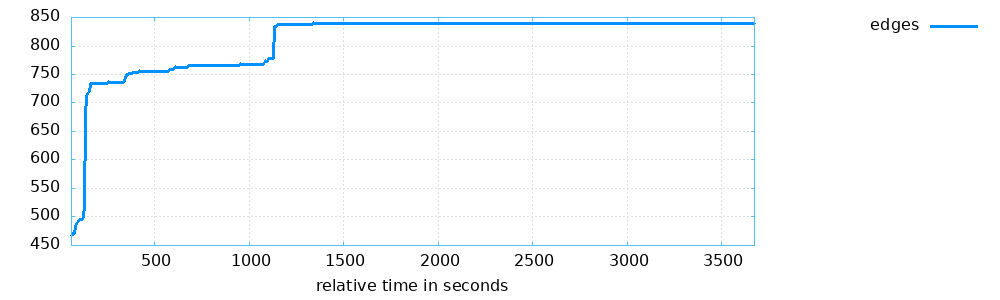
\includegraphics[width=\columnwidth]{Plots/run4_persistent/edges.png}
  \caption{Edges graph --- persistent mode. Full saturation reached at
  $\sim$$t$=1,200s (20~minutes); flat thereafter.}
  \label{fig:persistent-edges}
\end{figure}
 
\begin{figure}[h]
  \centering
  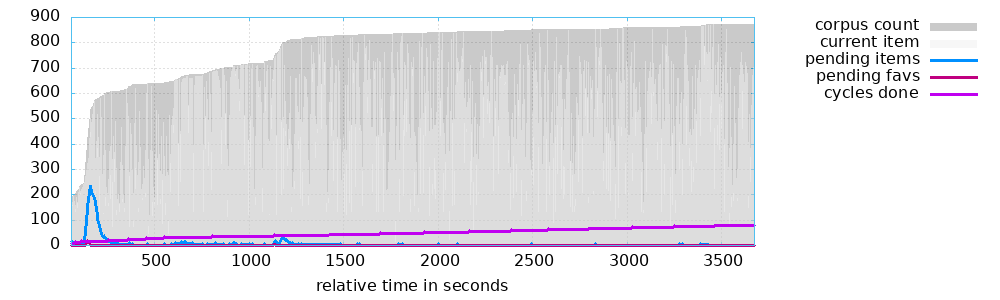
\includegraphics[width=\columnwidth]{Plots/run4_persistent/high_freq.png}
  \caption{Corpus and pending items --- persistent mode. Pending items
  exhausted by $t$=600s; 17 cycles completed.}
  \label{fig:persistent-high-freq}
\end{figure}
 
\begin{figure}[h]
  \centering
  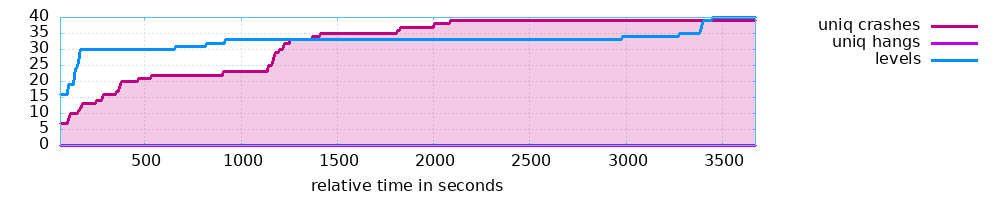
\includegraphics[width=\columnwidth]{Plots/run4_persistent/low_freq.png}
  \caption{Crashes and levels --- persistent mode. 77 unique crashes
  found, mostly within first 1{,}800s.}
  \label{fig:persistent-low-freq}
\end{figure}
 
\begin{figure}[h]
  \centering
  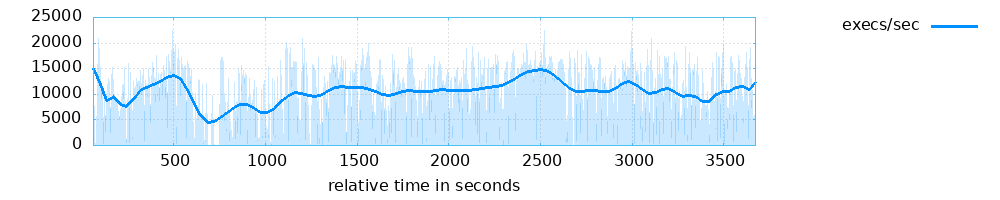
\includegraphics[width=\columnwidth]{Plots/run4_persistent/exec_speed.png}
  \caption{Execution speed --- persistent mode. Average
  $\sim$5{,}450 exec/sec throughout the run.}
  \label{fig:persistent-exec-speed}
\end{figure}

\newpage
\section{Comparison Table (Q8)}

\begin{table}[h]
\small
\begin{tabular}{llll}
\toprule
\textbf{Configuration} & \textbf{Exec/sec} & \textbf{Total execs} & \textbf{Speedup} \\
\midrule
No sanitizer + fork   & 4415   & 8.83M  & 5.16$\times$ \\
ASan + fork (baseline)& 855   & 1.71M  & --- \\
ASan + persistent     & 5450   & 10.9M & 6.37$\times$ \\
\bottomrule
\end{tabular}
\caption{Exec speed across three configurations (same seeds, same harness, 33 minutes).}
\label{tab:perf}
\end{table}

\end{document}